\documentclass[12pt]{article}
\usepackage{../../../lecture_notes}
\usepackage{../../../math}
\usepackage{../../../uark_colors}

\hypersetup{
  colorlinks = true,
  allcolors = ozark_mountains,
  breaklinks = true,
  bookmarksopen = true
}

\begin{document}
\begin{center}
  {\Huge\bf Midterm 2 - Fall 2025}
  
  \smallskip
  {\large\it ECON 4753 — University of Arkansas}
\end{center}

\vspace{5mm}
\begin{enumerate}
  \item In time-series data it is common to see the autocorrelation coefficient to decrease as you increase the order (e.g. $\rho_1$ to a 10-lag $\rho_{10}$). 
  Why is that common?
  
  \bigskip
  \item Say you are a news website trying to track the results of election polling. 
  For simplicity, say you observe a single election poll per day. 
  You want to present information on which candidate currently is in the lead.

  \medskip
  \begin{enumerate}[label=(\alph*)]
    \item Why might you want to use a moving average method (say exponential smoothing) to display the current leader of the race?

    \item As you approach election day, a lot of `undecided voters' will make up their mind. 
    To capture this in your simple exponential smoothing model, should you chose a relatively large or small value of $\alpha$? 
    Explain.

    \item Say you use a 15-day one-sided moving average. Comment on the quality of forecast this method might have for predicting who will win the election.
  \end{enumerate}

\end{enumerate}

\newpage
The following questions will involve time-series data on the \emph{weekly} number of wikipedia page views for Formula One (a sport involving car racing). 
See the next page for the figure and regression table.

\begin{enumerate}
  \setcounter{enumi}{2}
  \bigskip
  \item Say you have already ran a $2 \times 52$ MA to estimate the time-trend on the weekly data as displayed in the top plot of Figure \ref{fig:f1}. 
  Describe how you would estimate the seasonal trend, $\hat{S}_t$.

  \bigskip
  \item Now, say you wanted to run a time-series regression using this data. 
  You want to flexibly capture the trend in views over time so you can predict future popularity of the sport.
  \begin{enumerate}[label=(\alph*)]
    \item Why would you not want to use polynomials of the \texttt{date} variable to do this?
    
    \item What term(s) might you include instead?
  \end{enumerate}

  \bigskip
  \item The following questions will use the results of the time series regression displayed below. 
  The outcome variable is the \emph{log number of views}.

  \begin{enumerate}[label=(\alph*)]
    \item The variable \texttt{is\_race\_week} is an indicator variable denoting if the observation is a week where a race occurs. 
    Interpret the coefficient in words.
    Form a 95\% confidence interval of this coefficient.
    
    \item Which month has the largest number of views on average? 
    How do you know?
    
    \item Are the number of views trending upwards over time or not? 
    Is this a statistically significant relationship?

    \item Given the above time-series decomposition, we might have concerns that we are not fully capturing the trends in the time-series. 
    Why might it be useful to examine a plot of the regression residuals to assess this concern?

    \item At the end of the 2021 season, there was a large contreversy that resulted in a very large number of views for the month following the end of the season. 
    We do not want that incident to mess up our regression estimates. 
    What term could we include to fix this problem?
  \end{enumerate}
\end{enumerate}

\newpage
\begin{figure}[!th]
  \caption{Classical Decomposition of F1 Weekly Views}
  \label{fig:f1}
  
  \vspace*{-2\bigskipamount}
  \begin{center}
    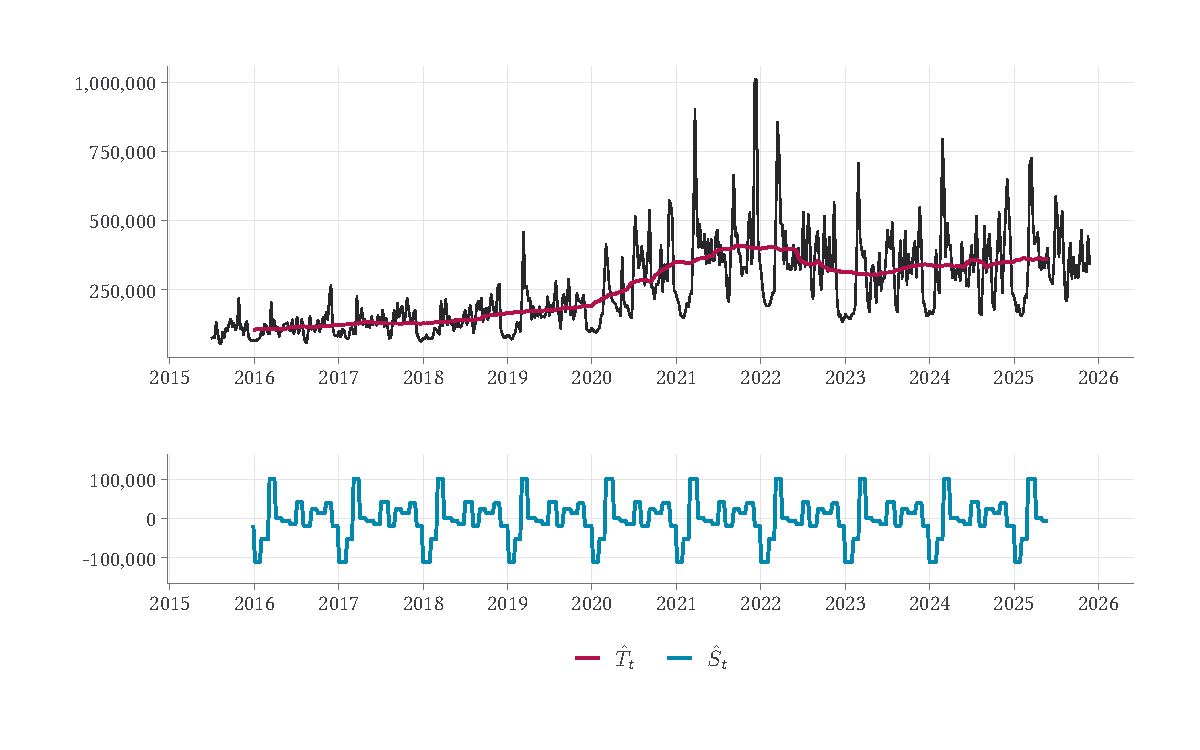
\includegraphics[width = 0.9\textwidth]{figures/p_f1_decomposition.pdf}
  \end{center}
\end{figure}

  \begin{smallcodeblock}[{}]
OLS estimation, Dep. Var.: log_views
Observations: 544
Standard-errors: Heteroskedasticity-robust
                  Estimate Std. Error t value   Pr(>|t|)
(Intercept)        -271.55      8.143   -33.3  < 2.2e-16 
year(date)            0.14      0.004    34.8  < 2.2e-16 
month::February       0.26      0.066     3.9 1.0985e-04 
month::March          0.70      0.071     9.9  < 2.2e-16 
month::April          0.42      0.059     7.1 4.6862e-12 
month::May            0.42      0.058     7.2 1.8021e-12 
month::June           0.33      0.059     5.6 3.4360e-08 
month::July           0.54      0.055     9.7  < 2.2e-16 
month::August         0.33      0.065     5.2 3.6351e-07 
month::Sepember       0.52      0.058     8.9  < 2.2e-16 
month::Octember       0.50      0.057     8.7  < 2.2e-16 
month::November       0.61      0.061     9.9  < 2.2e-16 
month::December       0.34      0.091     3.8 1.6936e-04 
is_race_week::TRUE    0.34      0.033    10.6  < 2.2e-16 
  \end{smallcodeblock}


\end{document}
